\documentclass[runningheads]{llncs}
\usepackage[T1]{fontenc}
\usepackage{algpseudocode, algorithm, amsmath, amssymb}					% packages to get the fonts, symbols used in most math
%\usepackage{dcolumn}
\usepackage[english]{babel}
\usepackage[hidelinks]{hyperref} % Add hyperlinks to references and citations
\usepackage{multirow}
\usepackage{latexsym}
\usepackage{listings}
\usepackage{booktabs}
\usepackage{tabularx} % For dynamic table width
\usepackage{parcolumns}
\usepackage{subcaption} % For sub-listings
\newcolumntype{C}{>{\centering\arraybackslash}X}
\renewcommand{\arraystretch}{1.5}
\usepackage{pifont} % For check and cross symbols
\newcommand{\cmark}{\textcolor{darkgreen}{\ding{51}}}  % Checkmark
\newcommand{\xmark}{\textcolor{red}{\ding{55}}}  % Cross
\newcommand{\mmark}{\textcolor{orange}{\ding{106}}}  % Cross

% T1 fonts will be used to generate the final print and online PDFs,
% so please use T1 fonts in your manuscript whenever possible.
% Other font encondings may result in incorrect characters.
%
\usepackage[dvipsnames,svgnames, table]{xcolor} % text color
\usepackage{graphicx}
% Used for displaying a sample figure. If possible, figure files should
% be included in EPS format.
%
\usepackage{svg}
\DeclareFontFamily{U}{mathx}{\hyphenchar\font45}
\DeclareFontShape{U}{mathx}{m}{n}{
      <5> <6> <7> <8> <9> <10>
      <10.95> <12> <14.4> <17.28> <20.74> <24.88>
      mathx10
      }{}
\DeclareSymbolFont{mathx}{U}{mathx}{m}{n}
\DeclareMathSymbol{\bigtimes}{1}{mathx}{"91}

% Define a style for the listings
\lstset{
    basicstyle=\ttfamily\small,
    numbers=left,
    numberstyle=\tiny\color{gray},
    backgroundcolor=\color{lightgray!20},
    frame=single,
    captionpos=b,
    numbersep=5pt, % Adjust space between numbers and code
    % framexleftmargin=10pt,             % Extend frame margin for line numbers
}


\DeclareRobustCommand{\ojoin}{\rule[0.10ex]{.3em}{.4pt}\llap{\rule[1.40ex]{.3em}{.4pt}}}
\newcommand{\leftouterjoin}{\mathrel{\ojoin\mkern-6.5mu\Join}}
\newcommand{\rightouterjoin}{\mathrel{\Join\mkern-6.5mu\ojoin}}
\newcommand{\fullouterjoin}{\mathrel{\ojoin\mkern-6.5mu\Join\mkern-6.5mu\ojoin}}

\newcommand{\cormark}[1]{\textsuperscript{#1}}

\definecolor{eclipseStrings}{RGB}{42,0.0,255}
\definecolor{eclipseKeywords}{RGB}{127,0,85}
\definecolor{darkgreen}{RGB}{0,128,21}
\colorlet{numb}{magenta!60!black}
\setlength{\parskip}{0pt}

% Packages
\usepackage[normalem]{ulem} % wavy underlines
\makeatletter
\def\uwave{\bgroup \markoverwith{\lower3.5\p@\hbox{\sixly \textcolor{red}{\char58}}}\ULon}
\font\sixly=lasy6 % does not re-load if already loaded, so no memory problem.
\makeatother

% Comments
%\newcommand{\todo}[1]{\noindent\textcolor{red}{{\bf \{TODO}: #1{\bf \}}}}
\newcommand{\TODO}[1]{\todo{#1}}
\newcommand{\citeneeded}{\textcolor{red}{{\bf [?!]}}}
\newenvironment{draft}{\color{gray}}{\color{black}}
\newenvironment{changed}{\color{black}}{\color{black}}

% todonotes
\usepackage{xargs}                      % Use more than one optional parameter in a new commands
\usepackage[colorinlistoftodos,prependcaption,textsize=tiny]{todonotes}
\newcommandx{\unsure}[2][1=]{\todo[linecolor=red,backgroundcolor=red!25,bordercolor=red,#1]{#2}}
\newcommandx{\change}[2][1=]{\todo[linecolor=blue,backgroundcolor=blue!25,bordercolor=blue,#1]{#2}}
\newcommandx{\info}[2][1=]{\todo[linecolor=OliveGreen,backgroundcolor=OliveGreen!25,bordercolor=OliveGreen,#1]{#2}}
\newcommandx{\improvement}[2][1=]{\todo[linecolor=Plum,backgroundcolor=Plum!25,bordercolor=Plum,#1]{#2}}
\newcommandx{\thiswillnotshow}[2][1=]{\todo[disable,#1]{#2}}
\newcommandx{\todoi}[2][1=]{\todo[inline,size=\small,linecolor=Plum,backgroundcolor=Periwinkle!25,#1]{#2}}
\newcommandx{\todoCite}[2][1=]{\todo[linecolor=Plum,backgroundcolor=Periwinkle!25,bordercolor=Plum,#1]{#2}}
\newcommandx{\todoDef}[2][1=]{\todo[linecolor=Plum,backgroundcolor=Periwinkle!25,bordercolor=Plum,#1]{Def.: #2}}



% Reviewers
\newcommand\olaf[1]{{\color{RoyalBlue}\textbf{Olaf}: #1}}


% Annotations
\makeatletter
\font\uwavefont=lasyb10 scaled 700
\def\spelling{\bgroup\markoverwith{\lower3.5\p@\hbox{\uwavefont\textcolor{Red}{\char58}}}\ULon}
\def\grammar{\bgroup\markoverwith{\lower3.5\p@\hbox{\uwavefont\textcolor{LimeGreen}{\char58}}}\ULon}
\def\phrasing{\bgroup\markoverwith{\lower3.5\p@\hbox{\uwavefont\textcolor{blue}{\char58}}}\ULon}
\let\rephrase\phrasing
\newcommand\ins{\markoverwith{\textcolor{LimeGreen}{\rule[-0.5ex]{2pt}{0.4pt}}}\ULon}
\newcommand\remove{\bgroup\markoverwith{\textcolor{red}{\rule[0.5ex]{2pt}{0.4pt}}}\ULon}
\makeatother

\algrenewcommand\algorithmicrequire{\textbf{Input:}}
\algrenewcommand\algorithmicensure{\textbf{Returns:}}


\lstdefinelanguage{sparql}{
    basicstyle=\tiny,
    keywordstyle=\color{eclipseKeywords},
    commentstyle=\color{blue}, % style of comment
    stringstyle=\color{darkgreen},
    keywords={FILTER, NOT, EXISTS, bound, OPTIONAL, BIND, IF, isIRI, AS, INSERT, UPDATE, DELETE, WHERE, SELECT, UNION, rr,rml,ql,rdfs},
    morecomment=[n]{?}{\ },
    morecomment=[l]\#,
    morestring=[b]",
    morestring=[s]{<}{>},
    frame=lines,
}
\lstdefinelanguage{rdf}{
    basicstyle=\tiny,
    keywordstyle=\color{eclipseKeywords},
    commentstyle=\color{gray}, % style of comment
    stringstyle=\color{darkgreen},
    keywords={rml, ql, rr, rdfs},
    morecomment=[n]{?}{\ },
    morecomment=[l]\#,
    morestring=[b]",
    morestring=[s]{<}{>},
    frame=lines,
}


\lstdefinelanguage{triples}{
    basicstyle=\tiny,
    keywordstyle=\color{eclipseKeywords},
    commentstyle=\color{darkgreen}, % style of comment
    keywords={a, rml, ql, rr, rdfs},
    morecomment=[s]{?}{\ },
    frame=lines,
}

  

% Set symbols % 
\newcommand{\symFragmentUniverse}{\mathcal{F}}
\newcommand{\symAttrUniverse}{\mathcal{A}}
\newcommand{\symTermUniverse}{\mathcal{T}}
\newcommand{\symAllStrings}{\mathcal{S}} % the symbol for the set of all strings
\newcommand{\symAllIRIs}{\mathcal{I}} % the symbol for the set of all IRIs
\newcommand{\symAllLiterals}{\mathcal{L}} % the symbol for the set of all literals
\newcommand{\symAllBNodes}{\mathcal{B}} % the symbol for the set of all blank nodes
\newcommand{\symRMLGraph}{G}
\newcommand{\symDataObjUni}{\mathcal{D}}
\newcommand{\symDataAccUni}{\mathcal{Q}}
\newcommand{\symDataSeqUni}{\bar{\mathcal{O}}}
\newcommand{\symAttrSubSet}{A}
\newcommand{\symProjSet}{P}
\newcommand{\symMappingTupleSet}{M}
\newcommand{\symRenamePFunc}{R}
\newcommand{\bigDataObject}{D}
\newcommand{\symSetDataset}{\mathcal{D}^\texttt{\tiny ds}\!}
\newcommand{\symSetDatasetX}[1]{\mathcal{D}^\texttt{\tiny ds}_{#1}}
\newcommand{\symSetContentA}{\mathcal{D}^\texttt{\tiny c1}}
\newcommand{\symSetContentAX}[1]{\mathcal{D}^\texttt{\tiny c1}_{#1}}
\newcommand{\symSetContentB}{\mathcal{D}^\texttt{\tiny c2}}
\newcommand{\symSetContentBX}[1]{\mathcal{D}^\texttt{\tiny c2}_{#1}}
\newcommand{\symDataAcc}{L}
\newcommand{\symDataAccX}[1]{L_{#1}}
\newcommand{\symDataSeqCard}[1]{D^{seq,#1}}
\newcommand{\symAttrQueryMap}{\mathbb{P}}
\newcommand{\symDataSeq}{\bar{O}}
\newcommand{\symExtExprSet}{E}
\newcommand{\symExtExprSeq}{\bar{\symExtExprSet}}
\newcommand{\symExtPairs}{\symExtExprSet}
\newcommand{\symTermSeqUniverse}{\bar{\symTermUniverse}}
\newcommand{\symFragmentPFunc}{\bbbf}
\newcommand{\symFragmentSet}{F}
\newcommand{\symJoinAttrPairs}{\mathbb{J}}
\newcommand{\symExtFuncUni}{\mathcal{E}}

% Special values % 
\newcommand{\card}{card}
\newcommand{\fragAttr}{a_\mathrm{frag}}
\newcommand{\fragDefault}{f_{0}}
\newcommand{\attr}{a}
\newcommand{\subjAttr}{\attr_\textrm{s}}
\newcommand{\predAttr}{\attr_\textrm{p}}
\newcommand{\objAttr}{\attr_\textrm{o}}
\newcommand{\graphAttr}{\attr_\textrm{g}}
\newcommand{\fragment}[0]{fragment}
\newcommand{\error}{\epsilon}
\newcommand{\mappingTuple}{t}
\newcommand{\symMappingInst}{I}
\newcommand{\mappingRel}{(\symAttrSubSet, \symMappingInst)}
\newcommand{\mappingRelSpec}[1]{(\symAttrSubSet_{#1}, \symMappingInst_{#1})}
\newcommand{\queryExpr}{q}
\newcommand{\rootIt}{rit}
\newcommand{\cobit}{cobit}
\newcommand{\dataObject}{d}
\newcommand{\eval}{\mathit{eval}}
\newcommand{\evalX}[1]{\eval_{#1}}
\newcommand{\cbeval}{\mathit{eval}'\!}
\newcommand{\cbevalX}[1]{\eval_{#1}'}
\newcommand{\sourceType}{type}
\newcommand{\sourceTypeX}[1]{type_{#1}}
\newcommand{\sourceTypeTuple}{(\symSetDataset, \symSetContentA\!, \symSetContentB\!, \symDataAcc, \symDataAcc'\!, \eval, \cbeval, \typeCast)}
\newcommand{\sourceTypeTupleX}[1]{\sourceTypeTupleXXX{#1}{#1}{#1}}
\newcommand{\sourceTypeTupleXXX}[3]{(\symSetDatasetX{#1}, \symSetContentAX{#2}, \symSetContentBX{#3}, \symDataAccX{#2}, \symDataAccX{#3}', \evalX{#2}, \cbevalX{#3}, \typeCastX{#1})}
\newcommand{\dataSource}{s}
\newcommand{\dataSourceTuple}{(\sourceType,\bigDataObject)}
\newcommand{\iterConfig}{\bbbc}
\newcommand{\sourceOp}[3]{\textrm{Source}^{(#1,#2,#3)}}
\newcommand{\sourceOpDflt}{\sourceOp{\dataSource}{\queryExpr}{\symAttrQueryMap}}
\newcommand{\sourceOpTuple}{(\dataSource, \iterConfig)}
\newcommand{\attrQueryPair}{(\attr \rightarrow \queryExpr)}
\newcommand{\typeCast}{cast}
\newcommand{\typeCastX}[1]{\typeCast_{#1}}
\newcommand{\length}{len}
\newcommand{\var}{v}
\newcommand{\indexSeq}{M}
\newcommand{\extExpr}{\varphi}
\newcommand{\extEval}{eval}
\newcommand{\extPairsType}{(\symAttrUniverse \setminus \symAttrSubSet) \times \symExtExprSeqUni}
\newcommand{\serdeAttr}{a_{serialized}}
\newcommand{\bgp}{\bbbb}
\newcommand{\extFunc}{f}
\newcommand{\extFuncType}{(\symTermUniverse \cup \{\error\})}
\newcommand{\extFuncTuple}{(\extFunc,\extExpr_1,\dots,\extExpr_n)}
\newcommand{\extOp}{\text{Extend}_{\varphi}^{\attr}}
\newcommand{\extOpAttr}[1]{\text{Extend}_{\varphi}^{#1}}
\newcommand{\renameOp}{\text{Rename}^{\symRenamePFunc}}
\newcommand{\equiJoinOp}{\text{Join}^{\symJoinAttrPairs}_{=}}
\newcommand{\triplesMapIRI}{u}
\newcommand{\triplesMapGraph}[2]{\symRMLGraph_{#1}^{#2}}
\newcommand{\toIRI}{\texttt{toIRI}}
\newcommand{\toBNode}{\texttt{toBNode}^{\LTB}}
\newcommand{\toLiteral}{\texttt{toLiteral}}
\newcommand{\template}{\texttt{template}^{\symAttrQueryMap}}
\newcommand{\initSrc}{\texttt{initSrc}}
\newcommand{\concat}{\texttt{concat}}
\newcommand{\concatSeq}{\texttt{concatSeq}}
\newcommand{\literal}{\ell}
\newcommand{\lex}{\mathit{lex}}
\newcommand{\dt}{\mathit{dt}}
\newcommand{\literalTuple}{(\lex, \dt)}
\newcommand{\LTB}{\mathit{L2B}}
\newcommand{\tempSubStrs}{\texttt{tempSubStrs}}
\newcommand{\substrSeq}{\bar{S}}
\newcommand{\projectOp}[1]{\text{Project}^{#1}}
\newcommand{\natJoin}{\text{NatJoin}}
\newcommand{\union}{\text{Union}}

% Functions % 
\newcommand{\fctDom}[1]{\mathrm{dom}(#1)}
\newcommand{\fctMappingTuple}[1]{\mappingTuple(#1)}
\newcommand{\fctAttrs}[1]{\mathrm{attrs}(#1)}
\newcommand{\fctCard}[2]{\card[#1](#2)}
\newcommand{\fctRootIt}[2]{\rootIt(#1, #2)}
\newcommand{\fctCobit}[3]{\cobit(#1, #2, #3)}
\newcommand{\fctEval}[2]{\eval(#1,#2)}
\newcommand{\fctEvalLang}[3]{\eval^{#3}(#1,#2)}
\newcommand{\fctCbeval}[3]{\cbeval(#1,#2,#3)}
\newcommand{\fctCbevalLang}[4]{\cbeval^{#4}(#1,#2,#3)}
\newcommand{\fctTypeCast}[1]{\typeCast(#1)}
\newcommand{\fctLength}[1]{\length(#1)}
\newcommand{\fctRenameTuple}[2]{rename^{#1}(#2)}
\newcommand{\fctSubst}[2]{subst^{#1}(#2)}
\newcommand{\fctExtFuncEvalN}[2]{\extFunc(\fctEval{#1_1}{#2},\dots,\fctEval{#1_n}{#2})}
\newcommand{\fctExtOp}[1]{\extOp(#1)}
\newcommand{\fctExtOpBig}[1]{\extOp\bigl(#1\bigr)}
\newcommand{\fctExtOpX}[3]{\text{Extend}^{#1}_{#2}(#3)}
\newcommand{\fctExtOpXBig}[3]{\text{Extend}^{#1}_{#2}\bigl(#3\bigr)}
\newcommand{\fctRenameOp}[1]{\renameOp(#1)}
\newcommand{\fctRenameOpBig}[1]{\renameOp\bigl(#1\bigr)}
\newcommand{\fctEquiJoinOp}[2]{\equiJoinOp(#1, #2)}
\newcommand{\fctEquiJoinOpBig}[2]{\equiJoinOp\bigl(#1, #2\bigr)}
\newcommand{\fctToIRI}[1]{\toIRI(#1)}
\newcommand{\fctToBNode}[1]{\toBNode(#1)}
\newcommand{\fctToLiteral}[1]{\toLiteral(#1)}
\newcommand{\fctTemplate}[1]{\template(#1)}
\newcommand{\fctImg}[1]{\mathrm{img}(#1)}
\newcommand{\fctInitSrc}[1]{\initSrc(#1)}
\newcommand{\fctConcat}[2]{\concat(#1, #2)}
\newcommand{\fctConcatSeq}[1]{\concatSeq(#1)}
\newcommand{\fctTempSubStrs}[1]{\tempSubStrs(#1)}
\newcommand{\fctProjectOpDflt}[1]{\fctProjectOp{\symProjSet}{#1}}
\newcommand{\fctProjectOp}[2]{\projectOp{#1}(#2)}
\newcommand{\fctProjectOpBig}[2]{\projectOp{#1}\bigl(#2\bigr)}
\newcommand{\fctNatJoin}[2]{\natJoin(#1,#2)}
\newcommand{\fctUnion}[2]{\union(#1,#2)}

% Layout %
\newcommand{\ttl}[1]{\texttt{\small #1}}  % for conrete IRIs, etc. used in examples and in formulas



%%%%%%%%%%%%%%%%%%%%%%%%%%%%%%%%%%%%%%%%%%%%%%%
% The following ensures that we have a (non-visible) table of contents embedded
% in the PDF, which PDF readers can show and, thus, allows me to navigate the
% document more easily.
%                                    Olaf
\setcounter{tocdepth}{3}
\hypersetup{bookmarksopen=true, citecolor=blue}
%
%%%%%%%%%%%%%%%%%%%%%%%%%%%%%%%%%%%%%%%%%%%%%%%


\begin{document}												% end of preamble and beginning of text that will be printed

\title{Bringing modern IDE features to Semantic Web formats with the Semantic Web Language Server}
%
%\titlerunning{Abbreviated paper title}
% If the paper title is too long for the running head, you can set
% an abbreviated paper title here
%
\author{Arthur Vercruysse\inst{1}\orcidID{0000-0003-3467-9755} \and
Julián~Rojas~Meléndez\inst{1}\orcidID{0000-0002-6645-1264} \and 
Pieter~Colpaert\inst{1}\orcidID{0000-0001-6917-2167}}
%

\titlerunning{The Semantic Web Language Server}
\authorrunning{A. Vercruysse et al.}
% First names are abbreviated in the running head.
% If there are more than two authors, 'et al.' is used.
%
\institute{
IDLab, Department of Electronics and Information Systems, Ghent University -- imec \\
\email{firstname.lastname@ugent.be}}
%
\maketitle              % typeset the header of the contribution
%

\begin{abstract}
% Context (What is needed to understand the "need"?)
The Semantic Web has introduced a variety of syntaxes for e.g., serializing, querying, and validating linked data, such as Turtle, SPARQL, and SHACL.
% Need (Why something needed to be done at all?)
While these formats enable powerful interactions with data, they are highly sensitive to human error; even minor typos can disrupt the semantics of a document, rendering it invalid or non-interoperable.
% Task (What was undertaken to address the need? It’s here that you write ‘in this paper, we …’)
% In this paper, we study how the authoring experience of Semantic Web documents can be enhanced through the use of the Language Server Protocol (LSP) with for instance code completion, syntax highlighting and live validation output.
% Object (What the present document does or covers)
In this paper, we demonstrate the Semantic Web Language Server (SWLS), an LSP implementation with features such as real-time syntax validation, context-aware autocompletion, and SHACL-based diagnostics to notify users of potential mistakes when interacting with Semantic Web documents.
% The language server is available as extensions for popular platforms like VS Code and Neovim, as well as in a standalone web-based interface (integrated into a Monaco editor).
% Findings (What the work done yielded or revealed)
By extending functionalities beyond what is already supported by the best-in-class YASGUI interface, our tool aims to further improve the development efficiency, precision, and confidence of power users, newcomers, domain experts, and data engineers.
% Conclusion (What the findings mean for the audience)
It integrates seamlessly into established Web-based and desktop development environments, and its layered architecture facilitates extending the code base to support new features in the future. 
% PC: This is a main track resource paper, not a workshop paper. Don’t promise an evaluation in future work.
% In future work, we will further extend feature support and perform user evaluations that allow us to identify improvement points. 
% Perspectives (What the future holds, beyond this work)
% This work not only addresses current limitations in semantic web tooling but also paves the way for broader adoption of semantic technologies by reducing barriers and improving usability.
\keywords{Language Server, IDE, Tool, End User Software Engineering, Semantic Web}
\end{abstract}

\textbf{URL:} \url{https://github.com/ajuvercr/semantic-web-lsp} 

\textbf{Licenses:} MIT License


\section{Introduction}%
\label{sec:introduction}

The Semantic Web comprises a variety of syntaxes for expressing and querying data, including Turtle, JSON-LD, and SPARQL. While these formats enable structured data representation and interoperability, they are prone to human errors, which can lead to validation failures or incorrect reasoning outcomes. For instance, mistyping the URI of a prefix can alter the entire meaning of a document, rendering it non-interoperable with other datasets. 

However, open services such as Linked Open Vocabularies (LOV)\cite{LOV2017} provide exact definitions of predicates and classes, offering a reliable reference for avoiding such errors.

In this paper, we introduce the \textbf{Semantic Web Language Server (SWLS)}, a language server designed to assist editors in handling semantic web documents. This demo paper accompanies an ESWC 2025 resource paper.

SWLS is not the only software that introduces IDE-like functionalities for Semantic Web documents. While tools such as YASGUI\cite{yasgui,10.1007/978-3-642-41242-4_7} and Query.wikidata.org provide robust web-based functionalities, they do not integrate seamlessly into local development environments or support a broader range of Semantic Web formats. In contrast, SWLS runs locally, allowing for quick development cycles and seamless integration into the developer's workflow. Moreover, SWLS supports multiple formats beyond Turtle it supports SPARQL and JSON-LD, making it a more versatile solution.

\section{Semantic Web Language Server}

SWLS follows the Language Server Protocol (LSP)\cite{IntroToLsp}\footnote{\url{https://microsoft.github.io/language-server-protocol/}}, a protocol designed by Microsoft to allow one server implementation to interact with different editors, reducing complexity from $O(M*N)$ to $O(M+N)$, where $M$ is the number of existing editors and $N$ the number of supported language implementations.

The server communicates using JSON-RPC, enabling bidirectional messaging between the editor and server for handling features such as autocompletion, validation, and diagnostics. Most modern editors support LSP, including Visual Studio Code and NeoVim.

SWLS is designed for flexibility, allowing support for multiple file formats with maximal code reuse. It uses an entity component system to build a layered architecture\cite{10.1145/3550355.3552452}, following a traditional \textit{Feature Execution Flow}. The ECS design enables reusing the \textit{Traverse} and \textit{Process} components across different languages, requiring only the \textit{Parse} step to be implemented separately per format.


In the \textit{Parse} step of the server handles parsing the document (emitting potential syntax errors) and deriving defined triples and prefixes.

The \textit{Traverse} step derives information from the triples, such as defined properties, classes and SHACL shapes, using Rudof\cite{labra2022rudof}. 
This step also fetches linked documents, like fetching the ontologies that are accessable with the defined prefixes, this uses the public LOV api, when these documents are fetched they are added to the ECS.

The \textit{Process} step extracts all required information for the current request and returns it to the editor.
Currently SWLS handles diagnostics (syntax and shape violations), autocompletion (predicates, classes and prefixes), renaming and hover.
 

\section{Demo}

\begin{figure}[tb]
    \centering
    \begin{subfigure}{0.48\textwidth}
      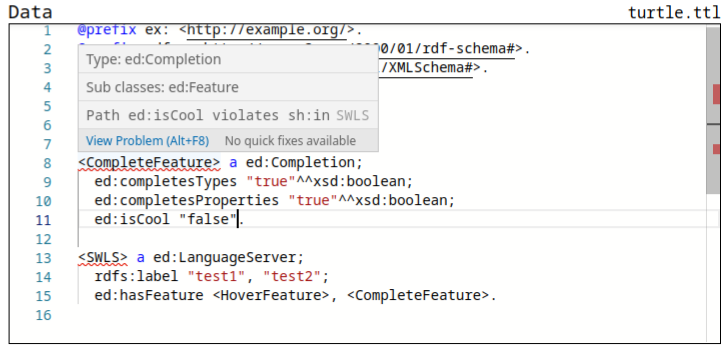
\includegraphics[width=\textwidth]{./images/hover.png}
      \caption{SWLS shows the user type information on hover as well as diagnostics}
      \label{hover}
    \end{subfigure}
    \hfill
    \begin{subfigure}{0.48\textwidth}
      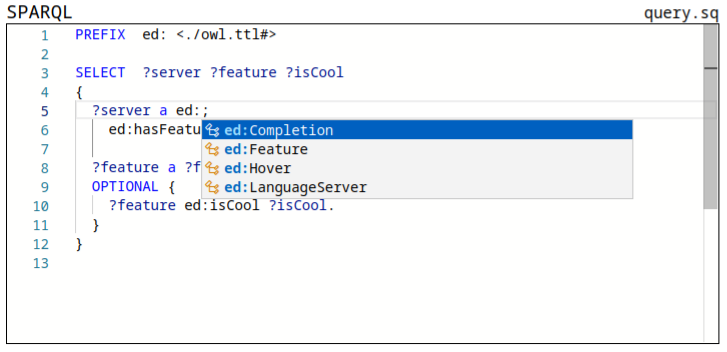
\includegraphics[width=\textwidth]{./images/class.png}
      \caption{SWLS completes a class when the user wants to write a class}
      \label{class_completion}
    \end{subfigure}
    \hfill
    \begin{subfigure}{0.48\textwidth}
      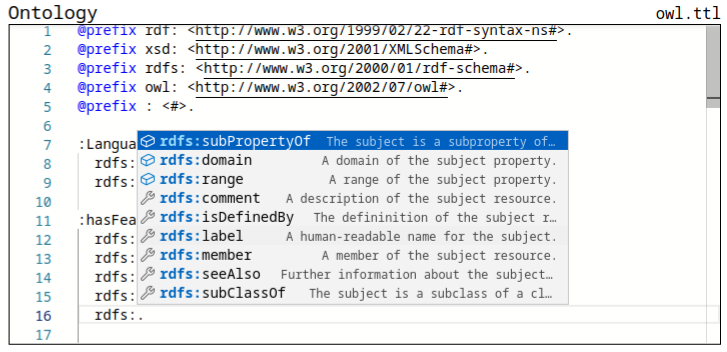
\includegraphics[width=\textwidth]{./images/property.png}
      \caption{SWLS completes properties, first the properties with the correct domain}
      \label{property_completion}
    \end{subfigure}
    \hfill
    \begin{subfigure}{0.48\textwidth}
      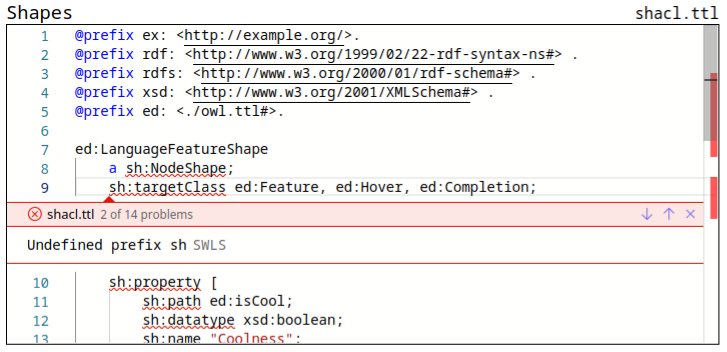
\includegraphics[width=\textwidth]{./images/undefined.png}
      \caption{SWLS notifies the user of undefined prefixes}
      \label{undefined_prefix}
    \end{subfigure}
    \caption{
      Demo application that shows the usage of SWLS. Features include hover information, autocompletion and diagnostics.
    }\label{lst:Demo}
\end{figure}

The demo consists of an online application at \url{https://ajuvercr.github.io/semantic-web-lsp/}.
The app has four editor panes each with a different purpose.
% : a data pane for authoring RDF data, an ontology pane for vocabulary management, a shape pane for SHACL constraints, and a query pane for SPARQL queries.
%
% All panes are treated equally, except for the query pane, which is designed for SPARQL rather than Turtle, but uses the same SWLS instance.

\begin{enumerate}
  \item The \textbf{data pane} presents an RDF dataset, where users can author and edit linked data. Errors detected via SHACL validation are highlighted, as shown in Figure \ref{hover}. Users can correct these errors either by adding missing triples or modifying the shape definitions in the shape pane.
  \item The \textbf{ontology pane} contains a playground ontology that describes language servers. It is linked to the data pane using a prefix import, enabling autocompletion of relevant properties, as shown in Figure \ref{property_completion}.
  \item The \textbf{query pane} allows users to write SPARQL queries against the data. While SWLS does not execute queries, it provides autocompletion for classes and properties, as depicted in Figure \ref{class_completion}.
  \item The \textbf{shape pane} includes SHACL constraints imported into the data pane via the \texttt{owl:imports} property. As shown in Figure \ref{undefined_prefix}, SWLS alerts users to undefined prefixes, and typing a prefix triggers autocompletion suggestions, simplifying corrections.
\end{enumerate}
% The main pane is the data pane, here some data about a language server is present.
% The user notices that two errors are present, coming from the shape validation, this is shown in Figure \ref{hover}.
% The user can fix this error by either adding the correct triples, or changing the shape in the shape pane.
%
% The ontology pane brings a play ground ontology that is used to describe language servers.
% The ontology is linked with the data pane with a prefix import, and enables autocompletion on properties, this is shown in Figure \ref{property_completion}.
% Properties that align with the domain are shown at the top.
%
% The query pane enables to user to write queries about the data.
% Note that there is no query exectuion support.
% In Figure \ref{class_completion}, autocompletion for classes is depicted.
%
% Lastly, the shape pane contains a SHACL shape with shape constrains.
% This shape is imported into the data pane with the \texttt{owl:imports} property.
% Figure \ref{undefined_prefix} shows that the language server notifies the user about undefined prefixes.
% To fix this, the user can start writing a prefix and is met with autocompletion suggestions, adding a prefix statement to the document.

Users can also try the language server on local editors.
For VSCodes, users can install the Semantic Web LSP\footnote{\url{https://marketplace.visualstudio.com/items?itemName=ajuvercr.semantic-web-lsp}}.
Using the language server with NeoVim requires installing the language server with cargo and configuring the language server with \textit{lspconfig}.

\section{Conclusion}

The Semantic Web Language Server (SWLS) introduces IDE-like functionalities for authoring Semantic Web documents, supporting multiple formats and providing a local development workflow. By integrating features such as real-time validation, context-aware autocompletion, and SHACL-based diagnostics, SWLS enhances the efficiency and confidence of both novice and experienced users. Unlike existing tools, SWLS runs locally and extends beyond SPARQL, offering a more flexible and powerful authoring experience. This work not only addresses current limitations in Semantic Web tooling but also paves the way for broader adoption of semantic technologies by reducing barriers and improving usability.





% \begin{credits}
% \subsubsection{\ackname} A bold run-in heading in small font size at the end of the paper is
% used for general acknowledgments, for example: This study was funded
% by X (grant number Y).
%
% \subsubsection{\discintname}
% It is now necessary to declare any competing interests or to specifically
% state that the authors have no competing interests. Please place the
% statement with a bold run-in heading in small font size beneath the
% (optional) acknowledgments\footnote{If EquinOCS, our proceedings submission
% system, is used, then the disclaimer can be provided directly in the system.},
% for example: The authors have no competing interests to declare that are
% relevant to the content of this article. Or: Author A has received research
% grants from Company W. Author B has received a speaker honorarium from
% Company X and owns stock in Company Y. Author C is a member of committee Z.
% \end{credits}

\bibliographystyle{splncs04}
\bibliography{./bibliography}

\end{document}
